\documentclass[sigplan,screen,10pt]{acmart}
\usepackage[utf8]{inputenc}
\usepackage{amsmath}
\usepackage{amsfonts}
%\usepackage{amssymb}
\usepackage{amsthm}
\usepackage{graphicx}
%\usepackage{xcolor}
%\usepackage{soul}
%\usepackage{hyperref}
\usepackage{algorithm}
\usepackage[noend]{algpseudocode}
%\usepackage{dsfont}
%\usepackage[font=small, labelfont=bf]{caption}
%\usepackage[left=2cm,right=2cm,top=2cm,bottom=2cm]{geometry}
\usepackage{subcaption}
\usepackage{todonotes}
\usepackage{multirow}
\usepackage{enumitem}
\newcommand\el[1]{\textcolor{orange}{{\bf Erick: }#1}}

\newcommand\ssbtokens[0]{\textit{SSB-Tokens} }
\newcommand\invpathcomment[0]{
\begin{flushleft}
{\color{commentgray}\textit{Msg} refers to enclosing SSB message. Properties (in italics) without an explicit access path refer to the operation properties stored in \textit{msg.content}. See implementation for other requirements not related to the paper arguments.} 
\label{req:comment}
\end{flushleft}}

\newcommand\idemcomment[0]{
\begin{flushleft}
{\color{commentgray} \textit{Idem} comment (see Req.~\ref{req:comment}).}
\end{flushleft}}

\newcommand{\mylabel}[2]{#2\def\@currentlabel{#2}\label{#1}}

\floatstyle{ruled}
\newfloat{invariants}{th}{inv}
\floatname{invariants}{Requirements}

\definecolor{commentgray}{gray}{0.28}

\hyphenation{block-chain}
\hyphenation{block-chains}
\hyphenation{Ethe-reum}


\copyrightyear{2022} 
\acmYear{2022} 
\setcopyright{rightsretained} 

\renewcommand{\copyrightpermissionfootnoterule}{%
\hrule
 \vspace*{-2pt}
  \noindent%
\\
\hfill
  
\includegraphics[width=0.20\columnwidth]{creative-commons-by_sa_4_0}
 \hfill
  \begin{minipage}[b]{0.75\columnwidth}
    \footnotesize 

This work is licensed under a \href{http://creativecommons.org/licenses/by-sa/4.0/}{Creative Commons Attribution-ShareAlike International 4.0 License}.
  \end{minipage}%
  \vspace*{2pt}%
\hrule
  \vspace*{2pt}
}


\acmConference[DICG'22]{3rd International Workshop on Distributed Infrastructure for Common Good}{Dec.  2022}{Montreal, Quebec, Canada}
\acmBooktitle{3rd International Workshop on Distributed Infrastructure for Common Good (DICG'22), December 2022, Montreal, Quebec, Canada}\acmDOI{XXX}
\acmISBN{XXX-X-XXXX-XXXX-X/XX/XX}

\begin{CCSXML}
<ccs2012>
   <concept>
       <concept_id>10010520.10010521.10010537.10010540</concept_id>
       <concept_desc>Computer systems organization~Peer-to-peer architectures</concept_desc>
       <concept_significance>500</concept_significance>
       </concept>
 </ccs2012>
\end{CCSXML}

\ccsdesc[500]{Computer systems organization ~Peer-to-peer architectures}

\keywords{economics, peer-to-peer, crypto-tokens, blockchain, local economies, producer credit, gossip algorithms}

\begin{document}


\title{SSB-Tokens: Efficient Secure Asset Gossip for Trust-Based Local Economics}

\author{Erick Lavoie}
\email{erick.lavoie@unibas.ch}
\affiliation{%
  \institution{University of Basel, Basel, Switzerland}
}

\author{Christian Tschudin}
\email{christian.tschudin@unibas.ch}
\affiliation{%
  \institution{University of Basel, Basel, Switzerland}
}


\begin{abstract}

\end{abstract}

\maketitle

\section{Introduction}

Major blockchain projects, such as Bitcoin (CITE) and Ethereum (CITE), implement \textit{global financial infrastructure}, respectively as a replicated ledger or as a state-machine. In both cases, creating new tokens, by forking an existing project or implementing them as smart-contracts, requires specialized technical skills. Moreover, maintaining the integrity of transactions demands Internet connectivity, and requires significant energy (CITE) or capital investment (CITE). The resulting costs become prohibitive for many applications that are inherently \textit{local} to a region or community.

For those applications, we propose instead to \textit{localize} the operations of crypto-token infrastructure in multiple complementary ways based on the following insights: (1) The creation of tokens is done by specific identities and authenticated, preventing any other identity to forge tokens for a different identity, foregoing the need for a global mining process; (2) The value of each specific token derives from the trust that its individual creator will fulfill the obligations they have linked to the tokens, instead of speculation on the future demand of a supply-limited token; (3) Transactions are public to a \textit{local} community, e.g. linked to a geographical region or bound by common interest, and recorded on identity-specific (immutable) append-only logs, instead of globally shared on a single global ledger; (4) Verification of the integrity of operations is done by each participant for the operations on which they depend, instead of having specialized miners performing the verification tasks for all participants; and, (5) Proofs of double-spending are immutable, linked to a specific identity, and the cost of fraud is ultimately the exclusion of that identity from participation in a community, which can be a greater loss than the potential gains obtained from fraud on common transactions. Compared to Bitcoin or Ethereum-based alternatives, localizing the operations simplifies the implementation of crypto-tokens and removes much of the technical or capital costs of maintaining transaction integrity. Instead our approach drastically reduces technical complexity and capital stakes with social trust and reputation, yet still enables a large variety of applications to be supported.

The main remaining technical challenge is to efficiently validate past operations, including ensuring that tokens were not spent more than once. To do so, each user is responsible for validating both the format and the availability of tokens they receive from others. 
%When validation fails, users can flag the incorrect transactions to remember and report them to others. Users that wrongly flag the transactions of others can be blocked from replication using the existing core operations of SSB and therefore excluded from future transactions. ß
As validity depends on an ever growing chain of transactions, we avoid verifying the same operations more than once by establishing a \textit{verification frontier} up to which all operations from a given user have been locally validated, effectively leveraging the \textit{total order} induced by append-only logs of Secure-Scuttlebutt~\cite{kermarrec2020gossiping}. Using a validation frontier instead of an explicit index of valid transactions lowers memory requirements.

%TODO: Discuss the benefits and challenges of using append-only logs for recording transactions. E.g. a log fork currently results in a partitioning of the SSB network, with implementations refusing to carry updates from the fork they do not carry. A proof-of-fork is recorded by publishing a message that links to both messages with the same sequence number. Because a user cryptographically signs their message, this acts as a proof of misbehaviour. For cases where the stakes are high enough to require proving that there are enough remaining tokens \textit{prior to the transaction}, a third trusted party can act as a \textit{witness}. Most commonly, the creator of the tokens has the incentive to do this but any other user can also do it.

In this paper, we build on the above insights to present \textit{an efficient system for secure asset gossip built on top of Secure-Scuttlebutt}. Specifically:
\begin{itemize}
 \item We present the design and implementation of \ssbtokens, a new crypto-token infrastructure that enables any user to securely issue their own tokens, send tokens to others, and flag invalid transactions, as well as efficiently validate previous operations through a \textit{validation frontier};
 \item  We present diverse applications that can be implemented with \ssbtokens  including fidelity cards, open source contribution tracking, crowdfunding of local projects, and token-supported mesh networking, showing the generality of our design;
 \item We show that our implementation can run on affordable hardware, such as Raspberry Pis. We test our system on real-world traces of transactions from ERC tokens showing that our implementation can support similar number of transactions and users, at reasonable processing time and storage.
\end{itemize}

In the rest of this paper, we motivate our design insights through a motivating example (Section~\ref{section:motivation}), we illustrate the problem of double-spending in replicated append-only logs (Section~\ref{section:double-spending}), we present the design of \ssbtokens (Section~\ref{section:design}), we present a variety of applications supported (Section~\ref{section:applications}), we evaluate the implementation on real-world transaction traces (Section~\ref{section:evaluation}), we compare to related projects (Section~\ref{section:related-work}) and finally conclude with future research directions (Section~\ref{section:conclusion}).

\section{Motivation: Fidelity Card in a Small Shop}
\label{section:motivation}

Consider a \textit{sandwich shop} that offers a fidelity card to its customers, with one stamp added on the card for each sandwich bought. After 10 stamps, customers can exchange the full card for a free sandwich. This is a common real-world business strategy we do not commonly associate with currencies, cryptographic or otherwise, and is therefore worth unpacking.

In effect, through this fidelity card program, the owner introduces a \textit{shop-specific currency}, that is only redeemable for sandwiches in his shop. Each token, in the form of an ink stamp made with a custom or hard-to-find rubber stamp,  is worth one-tenth of a sandwich and represents \textit{a promise} from the shop owner to offer sandwiches in the future in exchange for a sufficient number of tokens. A new token is \textit{created} every time a stamp is put on a card. The total supply of tokens has \textit{no a priori bound} and grows with the number of customers that choose to use the fidelity cards. In one particular example we found,\footnote{From private discussions with the \textit{Ty Chaud} shop owner in Grenoble (France): \url{http://tychaud.fr}.} the shop owner allows customers to redeem sandwiches using ten stamps collected in potentially multiple cards, even if the cards were partially filled by different customers: this effectively allows his customers to \textit{gift} their incomplete cards to others. Once a customer redeems a sandwich in exchange for cards worth 10 stamps, the owner destroys the card(s), effectively "\textit{burning}" the tokens that are on them. The lifetime of a token therefore ends with the destruction of the cards, either with the fulfillment of the underlying promise for a sandwich, or by destruction of the cards by others than the shop owner. Transactions with fidelity cards are instantaneous and free, and the material to run the program costs tens of Euros with no specialized skills.

\subsection{Comparison to Bitcoin and Ethereum}

Contrast the above to the operations of a Bitcoin or Ethereum infrastructure. In the case of Bitcoin, the tokens are created by \textit{miners} and there is an \textit{upper bound} on the total amount of coins in circulation. 
The value of Bitcoin is partially determined by its ability to store wealth and appreciate in value, based on growth in demand against a \textit{fixed number of tokens}. To use Bitcoins as tokens in a fidelity card, the shop owner would have to acquire them first in exchange for money. Acquiring tokens would take at least 10 minutes, and more likely at least 30 minutes to ensure enough blocks were confirmed, and transferring tokens to customers would require an Internet connection, transaction fees, and again 30 minutes of wait for confirmation. In the case of Ethereum, the shop owner could instead create one or multiple \textit{smart-contracts}, allowing the contracts to create as many shop-specific tokens as needed. However, transfers to customers would still require an Internet connection, transaction fees (in Ethereum tokens), and transfer confirmations would take at least a few minutes and up to an hour. Moreover, the creation of \textit{correct} smart-contracts requires programming skills that are beyond those of most shop owners. The costs of transactions and hourly wages to hire a programmer to maintain the fidelity cards would most likely consume all of the economic benefits of the fidelity card program. % Tokens are not usually intentionally destroyed, but may be lost or burned by sending to an invalid receiver address.

In effect, the Bitcoin and Ethereum-based financial infrastructures are ill-suited because they actually solve a different and much harder problem than is required for implementing a fidelity card program: both infrastructures achieve \textit{secure global transfers of tokens between untrusted parties}. In our shop example instead, the economic activity is \textit{local} and tied to a \textit{neighbourhood}, both limited in the geographical area it covers and the number of participants. There is no real need and little benefit to broadcasting fidelity card transactions to the entire world on a single ledger. The participants know each other, at least in their direct transactions with the sandwich shop. The value of tokens derives from \textit{trust} that the token emitter, \textit{e.g.}, the shop owner, will actually fulfill the associated promises in the future, \textit{e.g.} offer free sandwiches. 

A fidelity card program, made with paper cards and rubber stamps, is usually reserved for items of small value because it is not that difficult for customers to buy or create a similar rubber stamp and ink, and therefore \textit{forge} new tokens without actually buying sandwiches. However, with public-key cryptography and recent peer-to-peer gossiping systems, it is actually possible to achieve similar ease in token creation, fast transfers, and no transaction fees as in a fidelity card program but with stronger security properties: we can \textit{bind the tokens creation to a specific author}, such as the fidelity points created by a shop owner; (2) we can design other operations such that other participants \textit{cannot forge} new tokens but only refer to those created by the original author. We will present a design in Section~\ref{section:design} that achieves both. However, this is not sufficient to obtain a secure token system, because there can still be possibilities of \textit{double-spending}, i.e. transferring the same tokens to multiple participants, which we discuss next.

\section{Double-Spending in Append-Only Logs}
\label{section:double-spending}

To see how double-spending may arise, let's first consider a fidelity card program built on a gossiping system that replicates \textit{append-only logs}, such as Secure-Scuttlebutt (SSB)~\cite{kermarrec2020gossiping}. Participants have identifiers, written as \textit{@id}, which corresponds to their public key and they authenticate their messages with their corresponding private key, by signing the messages. Each new message signed also includes a pointer to the last message signed by the same \textit{author} and a strictly increasing \textit{sequence number} representing the index of the new message in the log.  

Figure~\ref{figure:example} shows one sequence of events between a customer and a shop owner illustrating transactions related to a fidelity card program.  The yellow boxes represent events happening in the real world, while the blue boxes represent \textit{operations} recorded on the logs, respectively of the shop owner (\textit{@shop}) and a regular customer (\textit{@customer}). In this example, the shop owner, in addition to giving a sandwich in exchange for $5$ Euros, also \textit{creates} then \textit{gives} a "Shop Point" to the customer. Once the customer has received 10 "Shop Points", she transfers the points to the shop owner to obtain a free sandwich. The shop owner then \textit{burns} the points, as the underlying promise of a free sandwich has been redeemed.

\begin{figure}[htbp]
\centering
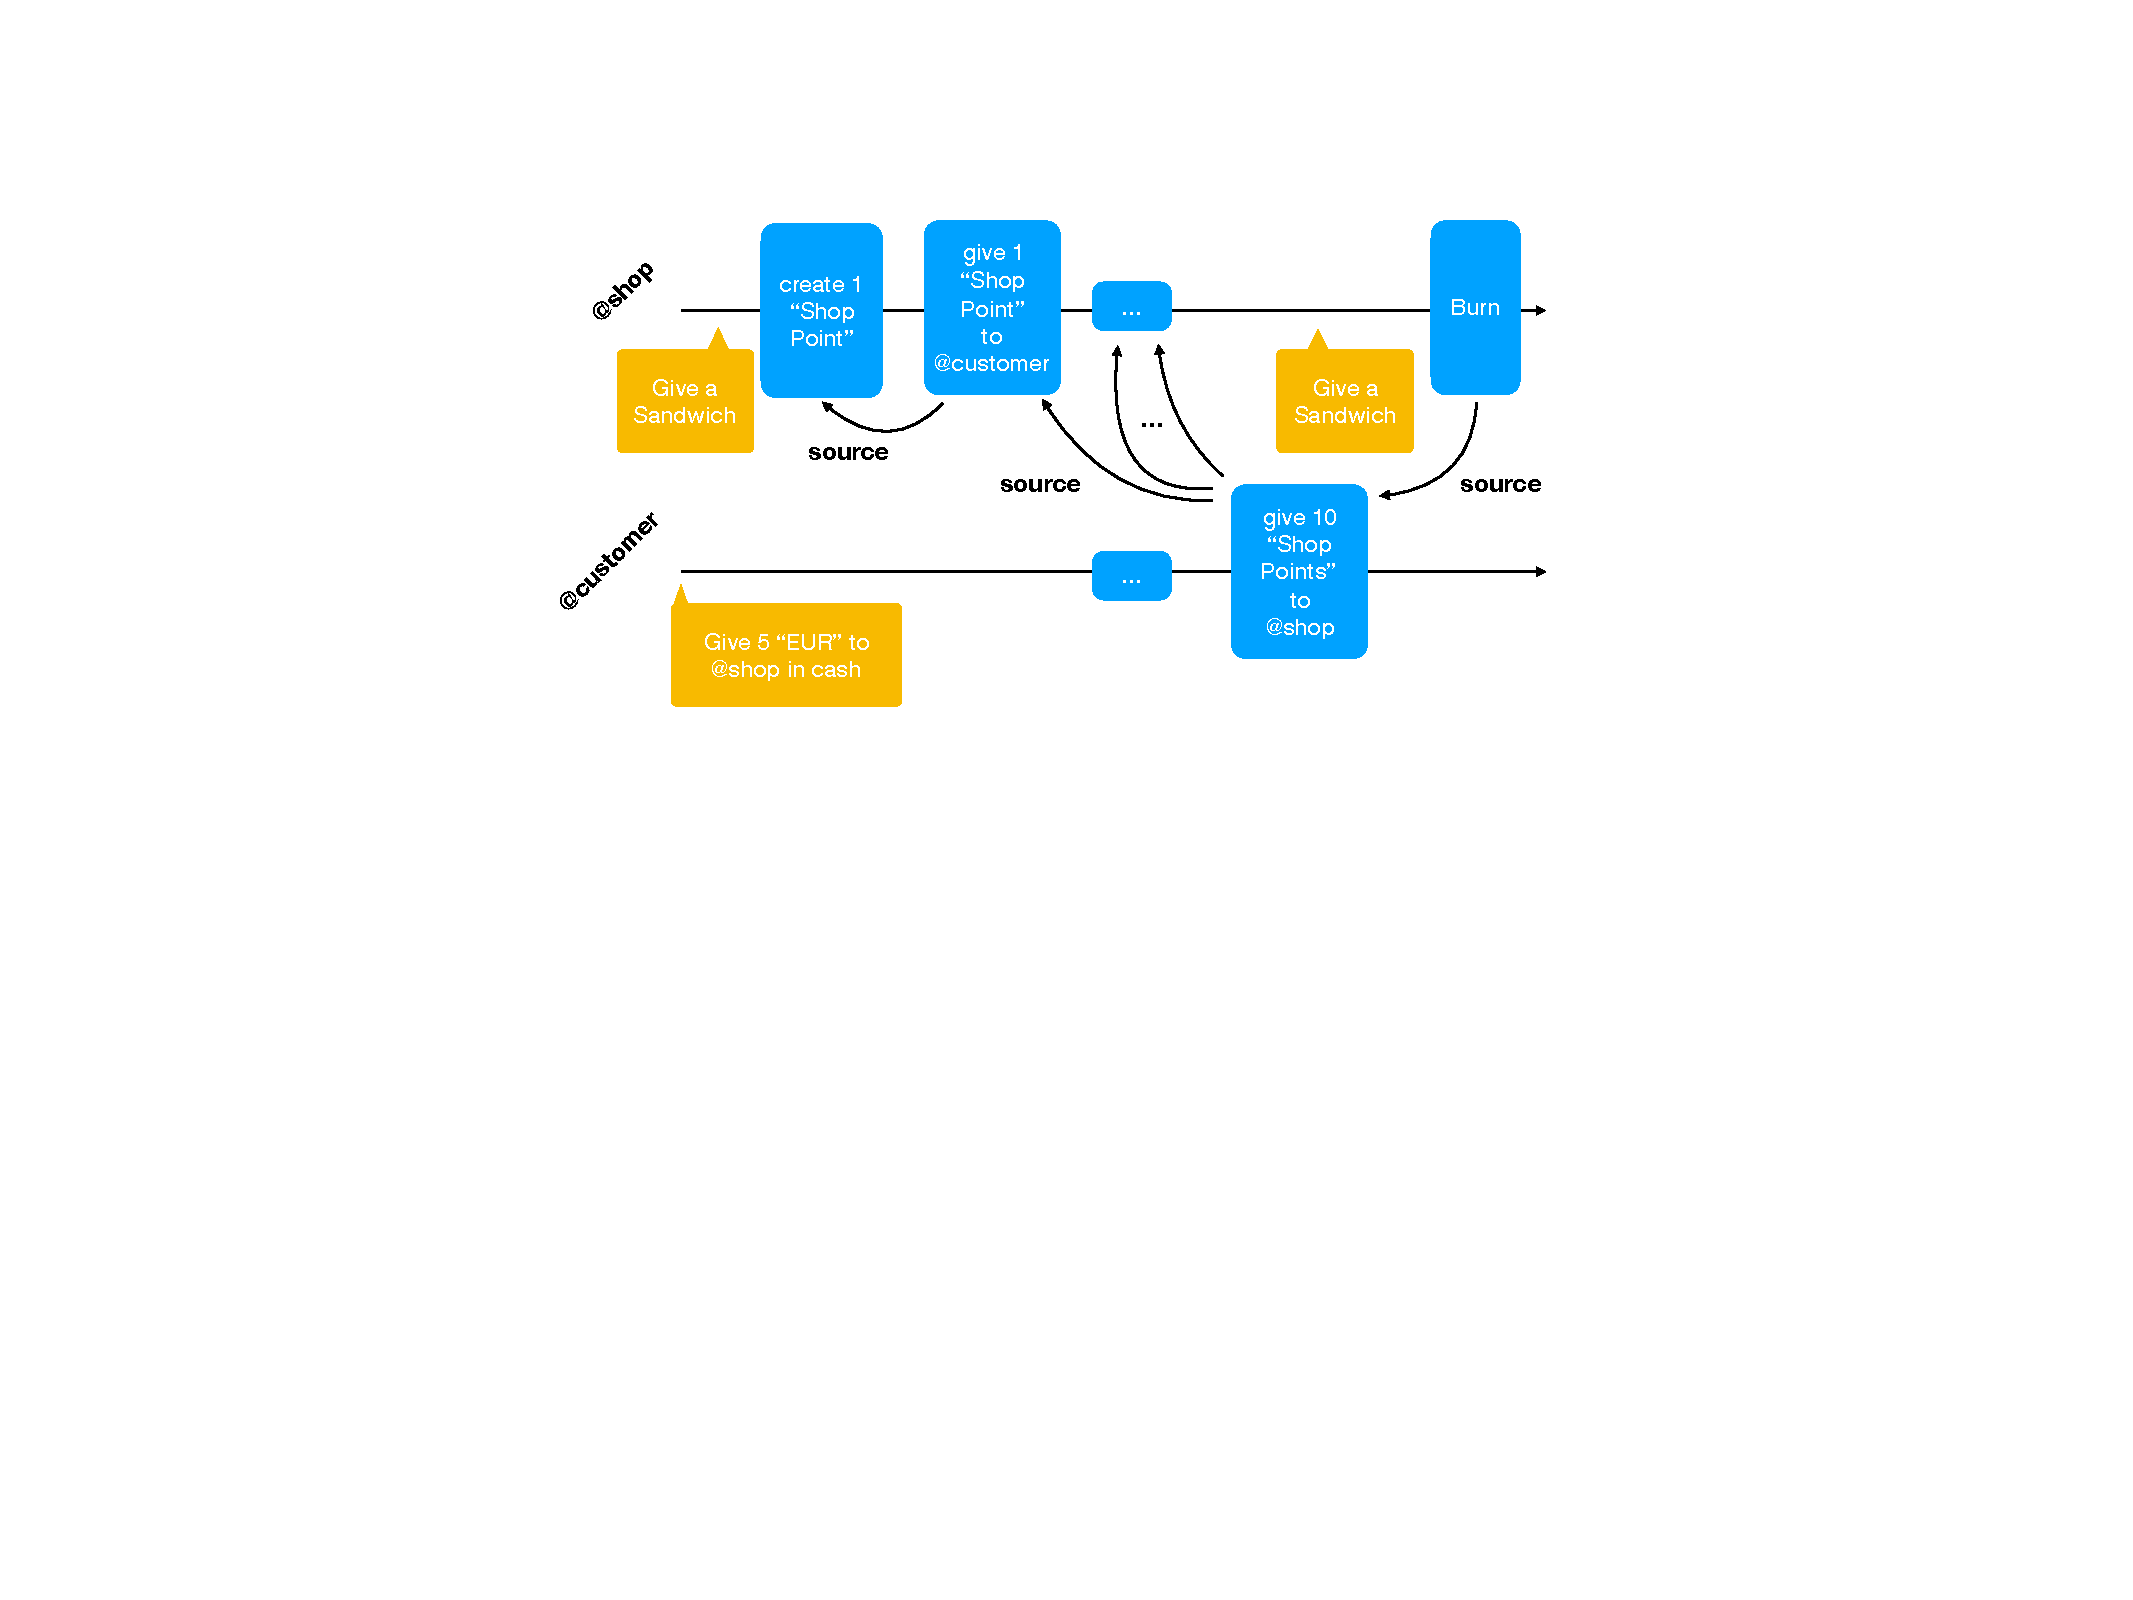
\includegraphics[width=0.40\textwidth]{./figures/example-src}
\caption{Example of \ssbtokens operations on SSB logs.}
\label{figure:example}
\end{figure}

Because participants are free to record any kind of operation in their logs, they may actually record operations in which they give the same tokens to multiple participants. Figure~\ref{figure:double-spend} illustrates one instance in which a customer gives the same tokens to two different participants, by using the same source in both operations. However, since both operations were immutably recorded in the customer log, and the messages were both signed by the customer, there is actually an \textit{immutable proof of double-spending}. This proof can be shared to other participants by \textit{flagging} all the operations that were involved in the fraudulent transactions. In this example, the first operation to \textit{@backer2} would be valid because up-to-that sequence number in the log, there was no double-spending. However, the second operation to \textit{@farmer} is  invalid because it spends tokens beyond what was available in the source. Because of the log structure, in which later messages point the earlier messages, there is a clear \textit{happened-before} relationship between the first and second transactions so we can discard only the second one.

\begin{figure}[htbp]
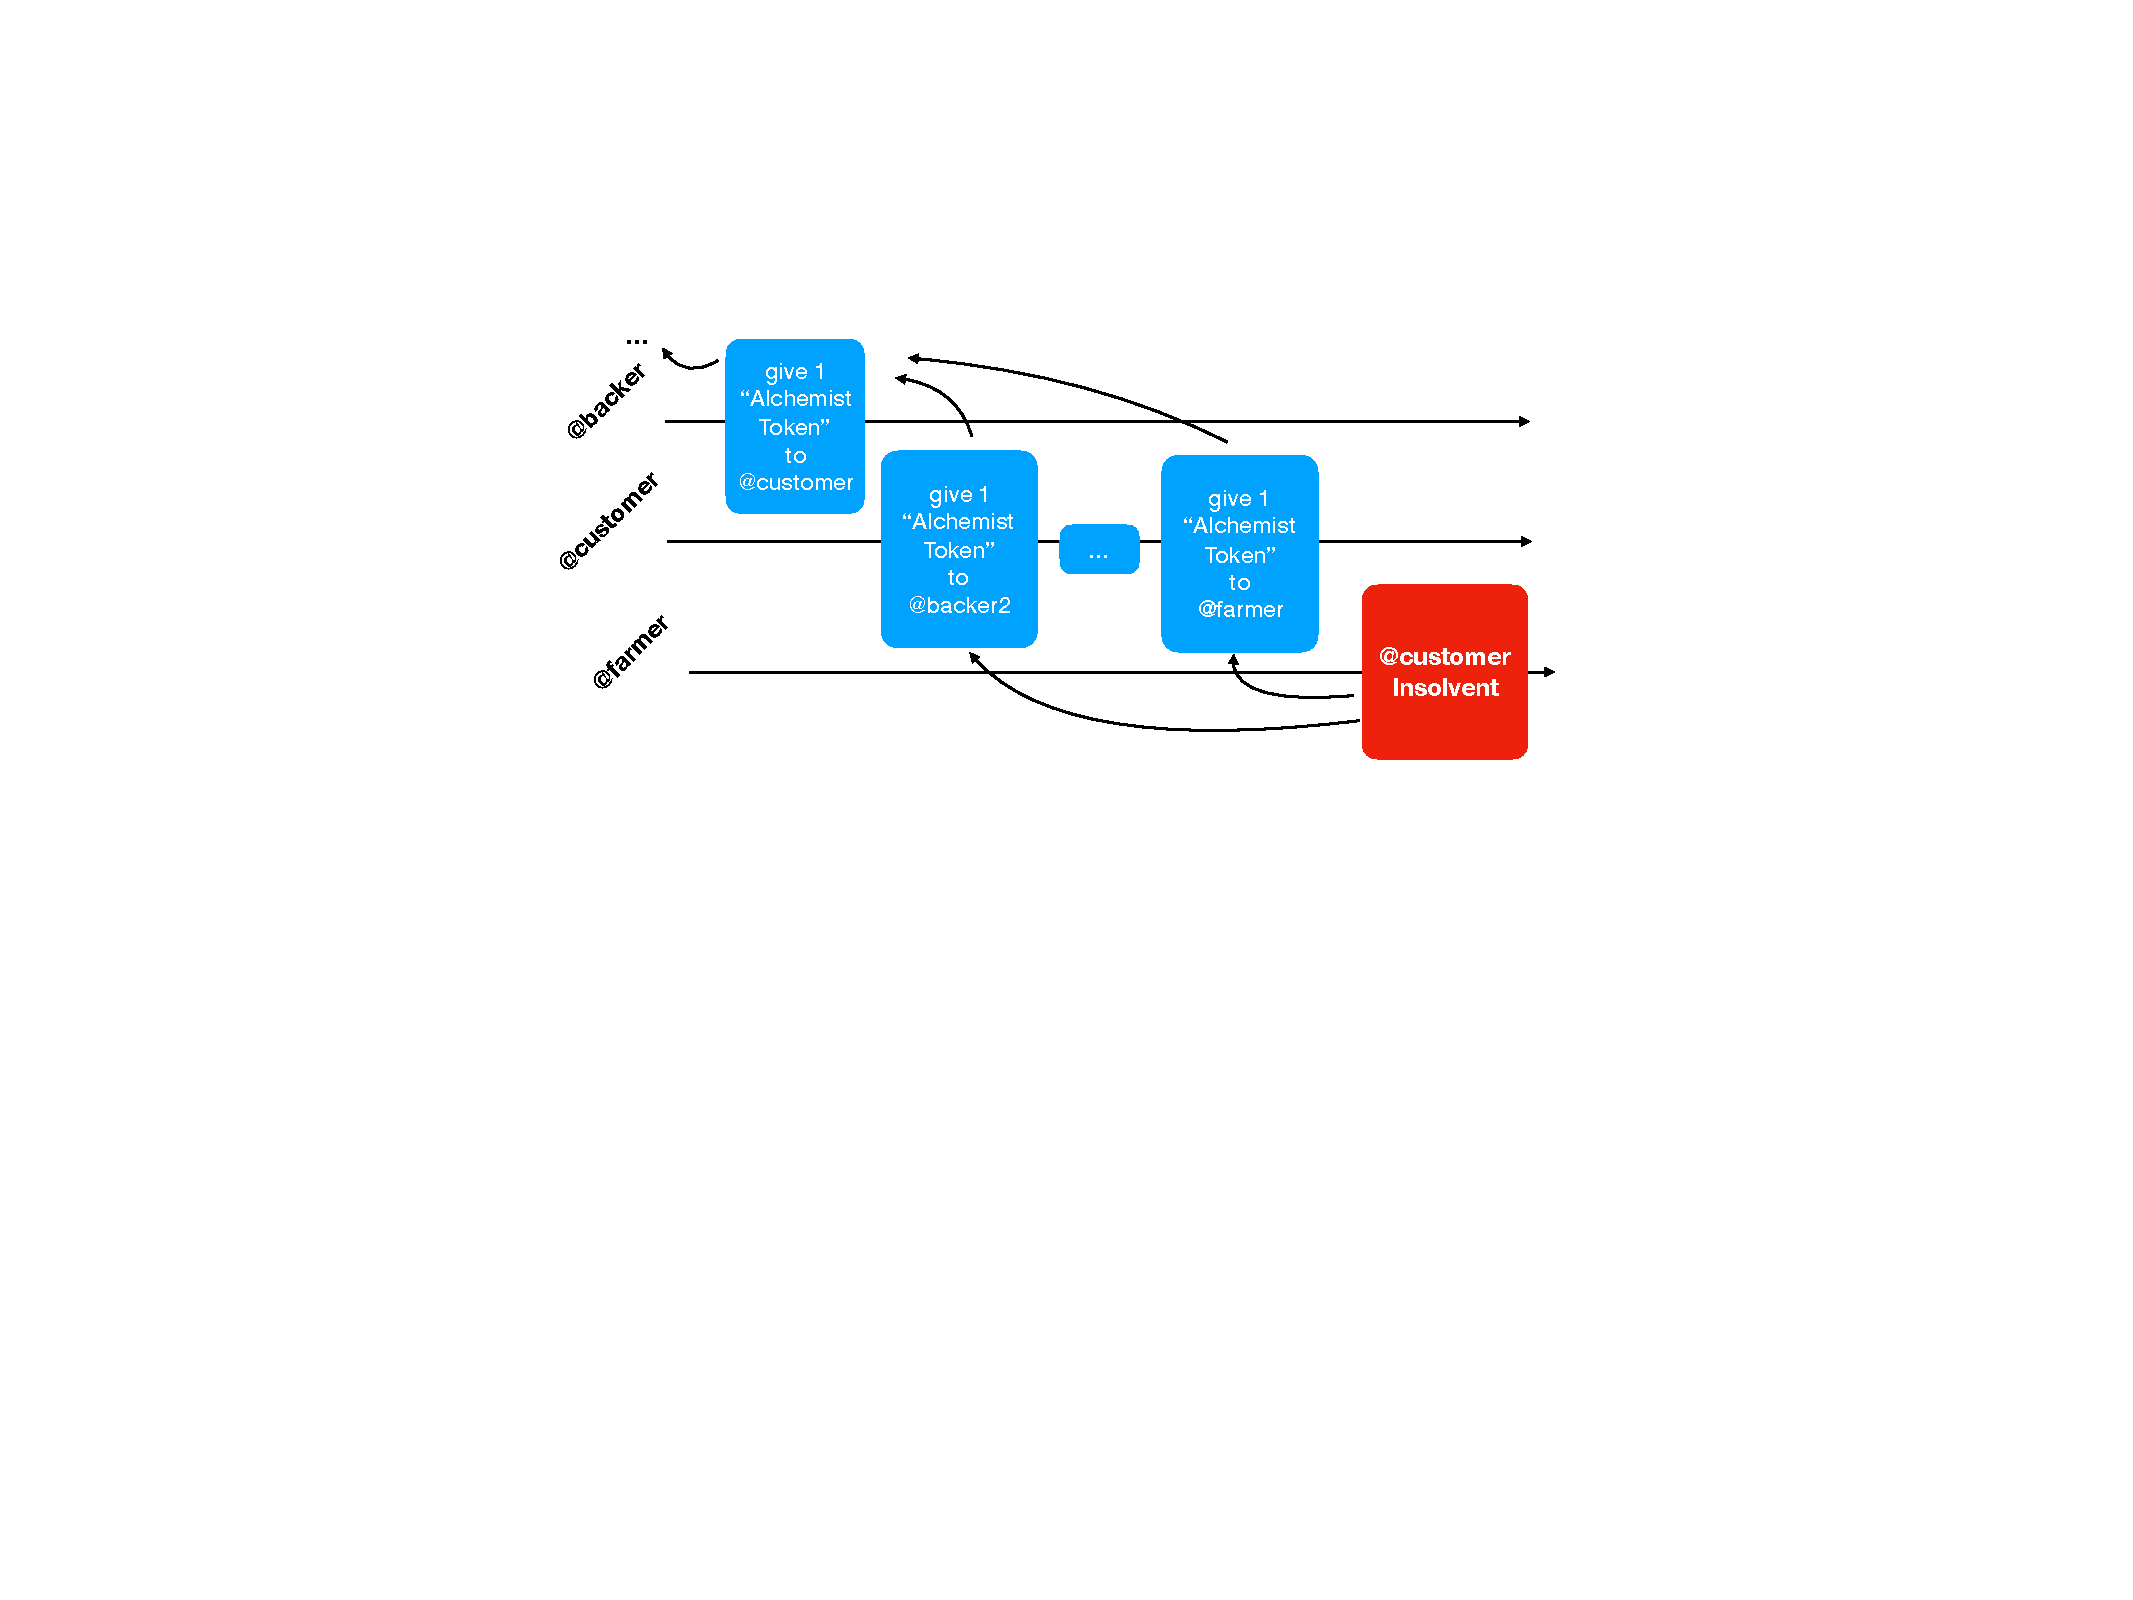
\includegraphics[width=0.45\textwidth]{figures/double-spend}
\caption{Double-Spend}
\label{figure:double-spend}
\end{figure}

A more subtle example of double-spending is illustrated in Figure~\ref{figure:fork-double-spend}, in which the customer presents \textit{different logs} to two other participants and can therefore rewrite the operation at sequence number 100 to give tokens twice, both to \textit{@farmer} and \textit{@backer}. This cannot be detected by other participants if they only have an interaction with \textit{@customer}. However, again because the messages are signed, eventually \textit{@farmer} and \textit{@backer} would replicate their local copy of \textit{@customer} log, either directly or through other participants in the community. The inconsistency will eventually be found ans it suffices to flag the identifiers of all messages creating new forks. In this case however, there is no clear \textit{happened-before} relationship between the two operations involved in double-spending, therefore both would be considered invalid.

\begin{figure}[htbp]
\centering
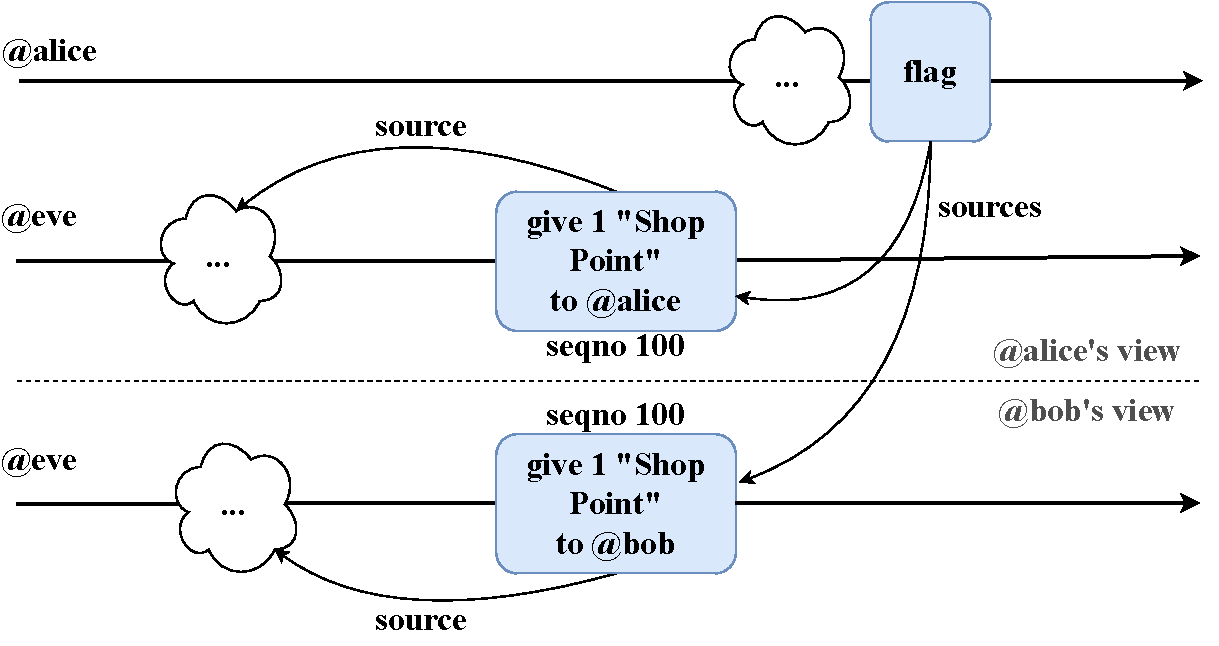
\includegraphics[width=0.45\textwidth]{figures/fork-double-spend}
\caption{Fork-based Double-Spending}
\label{figure:fork-double-spend}
\end{figure}

Moreover, a participant may fork their log at any time in the future, up to the first message of a log. Every time a fork is introduced, it invalidates all operations that happened after the fork. To invalidate any messages coming after, only the \textit{earliest} fork point need to be remembered, so the memory overhead is quite small. However, the recomputation of all operations rendered invalid may be prohibitive if forks happen frequently. The computation impact can be limited by rendering \textit{all} operations invalid coming from a log, for which more than two forks have been detected.\footnote{SSB currently does not support detecting forks. Instead participant's implementations refuse to replicate messages coming from the other side of a fork. This effectively creates a \textit{partition} between participants. A fraudster that would continue using one of the forks would have much trouble interacting with the rest of the community. This currently creates sufficient social incentives in the SSB community to \textit{not to fork their own log}, but would need to be addressed to carry higher stake token transactions.}  Generally, this also highlights the need to design a token system to limit the impact an adversary may have by crafting messages that deviate from normal operations.

In addition to the desired properties introduced at the end of Section~\ref{section:motivation}, our desired system should therefore properly deal with potential adversaries. In the next section, we extract from the previous discussions the desired properties of our alternative token system, \ssbtokens, and provide one design that implements them.

\section{SSB-Tokens}
\label{section:design}

\ssbtokens implements a \textit{secure asset creation and transfer gossip infrastructure} with the following properties, which follow directly from our previous discussions in Section~\ref{section:motivation} and~\ref{section:double-spending}:
\begin{enumerate}[label*=P.\arabic*]
	\item \textit{Creator-bound}: Tokens are bound to their creator (original author), with a unique type, even after transfers to others;\label{prop:author-bound}
	\item \textit{Unforgeable}: No author can create tokens for another author, and all transfers between participants use tokens that were explicitly created by an author; \label{prop:unforgeable}
	%\item[P.3] \textit{Consistent}: Operations that depend on other operations involve only tokens of the same type;
	\item \textit{Eventual double-spending detection and invalidation}: If two honest participants receive tokens from the same source with a total amount larger than what was originally available, the operations involved will be eventually detected by both participants. If some operations can be shown to have happened before the others, the earliest are valid and the latest invalid. Otherwise, all concurrent operations are invalid; \label{prop:double-spending-detection}
	\item \textit{Resilient}: Invalid operations cannot influence the derived state (e.g. token balance) computed from valid operations; \label{prop:resilient}
	\item \textit{Limited adversary resource impact}: An adversary may induce additional Memory or CPU consumption on honest participants by creating invalid messages or forking their log. However, for commonplace situations this should have limited impact, and for exceptional cases, be sufficiently costly for an adversary to be disincentivized. \label{prop:bounded-adversary-impact}
	%higher than a fixed (low) bound. \label{prop:bounded-adversary-impact}
\end{enumerate}

Compared to Bitcoin and Ethereum, our design \textit{does not prevent double-spending} and instead detects and invalidates incorrect operations after the fact. Techniques for prevention, such as relying on third-parties to act as witnesses~\cite{guerraoui2021consensus,otte2020trustchain}, are compatible and complementary to our design, but in general they require an Internet connection and online peers. In this paper, we instead rely on \textit{reputation loss} induced by the detection of fraud, and the potential to be excluded from participation in a community, as disincentive. This is sufficient as long as the benefits of double-spending are less than the loss induced by community exclusion, which is the case for the kind of \textit{local} applications we are targetting (Section~\ref{section:applications}).

In the remainder of this section, we present the full design of \ssbtokens and show that the design indeed implements the properties above. 


\subsection{System Model}
\label{section:system-model}

\el{Capabilities of adversary?}

First, we assume a fully asynchronous environment between any two nodes, i.e. that a message created by a node may take an arbitrary long time before being replicated on any other node. We further assume any message will eventually be replicated by all participants.\footnote{The implementation of SSB requires a stronger assumption for synchronization between a pair of temporarily-connected replicas: it actually relies on partial synchrony, i.e. that most messages will be delivered before a timeout between two nodes. However, it may take an arbitrary long time for any two pair of nodes to contact and connect to each other to replicate messages, therefore from an application perspective the infrastructure operates in an asynchronous environment.} This property enables eventual detection of double-spending (\ref{prop:double-spending-detection}).

Second, every node has an identity that corresponds to the public key of the public-private key pair that is used for signing messages, which guarantees that messages cannot be forged by nodes that don't have access to the corresponding private key. Messages are organized in an append-only log, i.e. an immutable list that can only be extended but never updated, authenticated by a single identity. This property enables binding the creation of tokens to an author (\ref{prop:author-bound}), and the detection of double-spending (\ref{prop:double-spending-detection}). The last two properties are provided by the underlying SSB implementation~\cite{kermarrec2020gossiping}.

Third, we assume that every node has enough storage to replicate all messages from other nodes within their community. As shown in Section~\ref{section:storage}, current common devices can store messages from \el{Empirical number X}s of users, which should be sufficient for most local applications. This property enables validation of the complete history of operations on which a participant depend, to provide \ref{prop:double-spending-detection}.

Fourth, for presentation simplicity, we assume a single node and its identity correspond to a single physical person and that all activity of that person are recorded on the same log. However, in practice, implementations may allow different applications for the same person to segregate their messages in different logs without loss of generality. A log may also be updated following synchronization between different physical persons through an out-of-band protocol so that the log may represent a collective identity,  but this is out-of-scope of this paper and not covered by SSB's core operations at the time of writing.

\subsection{Message Format and Semantics}


\footnotetext{This is a simplified (two-level) schema to improve the readability of algoritms. The actual SSB JavaScript implementation instead uses three levels: \textit{msg.key} is on the first level; all other properties are on a second level under \textit{msg.value}; and the application content is on the third level under \textit{msg.value.content}. The three levels make it clearer that the key to identify a message is derived from the content of \textit{msg.value} but introduce unnecessary verbosity when presenting our algorithms.}

All our messages are stored as content of SSB messages (Figure~\ref{fig:ssb-message-schema}). Notably, for a given message \textit{msg}, its identifier is accessible through \textit{msg.key}, its author as \textit{msg.author}, its sequence number as \textit{msg.sequence}, its ancestor in the log as \textit{msg.previous}, and its content as \textit{msg.content}.


\begin{figure}[ht]
\flushleft
\texttt{ msg = \{ 
     "key": \textbf{SSBMsgId},
     "author": \textbf{SSBLogId}, 
     "sequence": \textbf{Number}, 
     "previous": \textbf{SSBMsgId} || \textbf{null},  
     "content": \textbf{Object},
     "signature": \textbf{String}
\} 
     }
\caption[]{SSB message schema (JSON notation augmented with types in bold). Application messages are stored in \textit{msg.content}.\footnotemark }
\label{fig:ssb-message-schema}
\end{figure}


\begin{table*}[t]
\centering
\caption{Format of \ssbtokens operations (JSON notation augmented with types in bold), stored in \textit{msg.content} of a SSB message.}
\label{table:api}
\begin{tabular}{|l|l|} 
\hline
\textbf{\ssbtokens  Operation Types}          & \textbf{Semantics}                                                                                                           \\ 
\hline
\begin{tabular}{@{}l@{}}
\texttt{\{ "type": "tokens/create", "amount": \textbf{Number},}  \\
\texttt{"name": \textbf{String[30]}, \texttt{"unit": \textbf{String[10]},}}\\
\texttt{"decimals": \textbf{Number}, "description": \textbf{SSBMsgId},}\\
\texttt{ "tokenType": \textbf{String[16]} \}} ß\\
\el{Add bloom filter for token properties to find more efficiently.}
\end{tabular} ~& 
\begin{tabular}{@{}l@{}}Create \textit{amount} tokens identified by \textit{name},\\
 denominated in \textit{units}, which can be sub-divided \\
 in at most \textit{decimals}, binding creator  (\textit{msg.author}) \\
  to  promises in \textit{description}. 
\end{tabular}                                  \\ 
\hline
\begin{tabular}{@{}l@{}}
\texttt{\{ "type": "tokens/give", "sources": [ \{ "amount": \textbf{Number},} \\
\texttt{ "id": \textbf{SSBMsgId} \}, ... ], "receiver": \textbf{SSBLogId}, } \\
\texttt{"amount": \textbf{Number}, "tokenType": \textbf{String[16]}  \}}     
\end{tabular}
& Give \textit{amount} tokens from \textit{sources} to \textit{receiver}.                                                                 \\ 
\hline
\begin{tabular}{@{}l@{}}
\texttt{\{ "type": "tokens/burn", "sources": [ \{ "amount": \textbf{Number},} \\
\texttt{ "id": \textbf{SSBMsgId} \}, ... ], "amount": \textbf{Number}, } \\
\texttt{"tokenType": \textbf{String[16]}  \}}    \\
\el{Add bloom filter for quick sources membership filtering.}
\end{tabular}             & Destroy tokens from \textit{sources}.                                                                                             \\ 
\hline
\begin{tabular}{@{}l@{}}
\texttt{\{ "type": "tokens/flag", "sources": [ \textbf{SSBMsgId}, ... ],} \\
 \texttt{ "label": \textbf{String[30]},"tokenType": \textbf{String[16]} \}} 
 \end{tabular}      &  
 \begin{tabular}{@{}l@{}}
 Assign a flag with \textit{label} on \textit{sources}. \\
 \end{tabular}                             \\ 
\hline
\begin{tabular}{@{}l@{}}
\texttt{\{ "type": "tokens/unflag", "flag": \textbf{SSBMsgId},} \\
\texttt{"tokenType": \textbf{String[16]} \}}    
\end{tabular}
 & \begin{tabular}{@{}l@{}}Remove a previously assigned \textit{flag}.  \end{tabular}                               \\ 
\hline
%\texttt{list(tokenType :String, owner :SSBLogId)}          & \begin{tabular}{@{}l@{}}List the current state of token, identified \\ by \textit{tokenType}, owned by \textit{owner}.   \end{tabular}                             \\ 
%\hline
%\texttt{validate(amount :Number, src :SSBMsgId)}    & \begin{tabular}{@{}l@{}}Validate that \textit{src} has \textit{amount} \\ available and all transitive sources are valid. \end{tabular}  \\
%\hline
\end{tabular}
\end{table*}

All of \ssbtokens operations are stored as the \textit{content} of SSB messages. To distinguish clearly between the two levels, we use \textit{message} and the abreviation \textit{msg} to refer to SSB messages, and \textit{operation} to refer to the content of SSB messages that represent \ssbtokens operations. Moreover, operations implicitly reuse some of the fields of SSB messages to avoid redundancy: their \textit{identifier} and \textit{author} are the same as the identifier and author of SSB messages that contains them.\footnote{The application programming interface of \ssbtokens assigns both properties respectively as \textit{id} and \textit{author} on returned objects representing the operations, to abstract from the underlying SSB storage format.}

\el{Unformize presentation of burn and give}

Table~\ref{table:api} shows the syntactic format of \ssbtokens operations and their associated semantics. The core of \ssbtokens is organized around \texttt{create}, an operation that creates a certain number of tokens, associated specifically to their creator; \texttt{give}, an operation to transfer a subset of tokens from one or multiple sources to another user; and \texttt{burn} an operation to destroy all tokens from a given (owned) source, for example, when another user has redeemed the real-world underlying value represented by the token.  Note that the give operation is unilateral, i.e. it does not require acceptance by the recipient to be effective. In case a recipient receives tokens they did not want, they can block the sender or burn the tokens. Notice also that a \texttt{burn} should destroy the entire original amount of tokens in their sources. This simplifies reasoning about tokens flows, as only the \texttt{give} operation can split a source into many. Shall a partial burn be need, a user can first give a partial amount of a source to themselves then burn the new give operation.

In addition to the core operations for manipulating tokens, \texttt{flag} and \texttt{unflag} enable users to assign (and remove) labels to recorded operations. This can be useful, for example, to share that a user found invalid messages in other logs, or to enable the creator to cancel tokens that are circulating, or ask their owners to return them in exchange for newer valid tokens. The validation of past operations (Alg.~\ref{alg:validation}) does not rely on flags, only the format and values of messages for core operations, to prevent malicious users from tempering with the validation process. However, the labels may still alert other users to invalid operations and focus their validation efforts on those first to verify for themselves that they were indeed invalid. After a second validation that was inconsistent with the flags applied by malicious users, a user may decide to block the authors of invalid flags using the core operations of SSB~\cite{kermarrec2020gossiping}. The label of flags is user-defined enabling users to find additional uses beyond the two precendent.

% The \texttt{flag} and \texttt{unflag} operations are used for multiple uses. First, the creator of the tokens can \textit{cancel} tokens in circulation that have not yet been returned, to signify that the associated promise won't be honored. Second, receivers of invalid tokens, e.g. they were incorrectly formatted or the associated source did not have a sufficient remaining balance, can report the incorrect operations to exclude them from available funds locally and warn others that the operations may be incorrect. In addition, the \textit{label} field is user-defined to enable other potential user applications.

In addition, to their specific fields, all messages (but \texttt{unflag}) include an  an additional \textit{tokenType} property. The \textit{tokenType} makes it faster to query for all related messages, without having to first recursively retrieve the corresponding \texttt{create} messages through a transitive list of sources. As shown later in the invariants of a \texttt{create} operation (Alg.~\ref{alg:create}), the \textit{tokenType} combines all attributes of the token (name, unit, description, and smallest unit) with its author, making the hash (and identity) of a token specific to an author and unique among all tokens.

\subsection{Requirements on Operation Values}
\el{Replace "smallestUnit" with "decimals"}
\el{Clean-up discussion on requirements not strictly necessary for the argument.}\

In this section, we explicit all the requirements on operation values, in addition to the syntax listed in Table~\ref{table:api}, for operations to be considered valid\footnote{For clarity of presentation, all requirements that do not derive from JSON structure and types are listed together. The implementation however splits the checks according to their performance costs: all requirements that can be checked without a lookup are performed in the \textit{validate.format} method, while all those that require a lookup are performed in the \textit{validate.requirements}.}. The list is used for two purposes: first to validate user inputs as part of the API prior to publishing corresponding messages on SSB, and, second, to validate messages published by other users, as we have no guarantee that their implementation of \ssbtokens actually follows the same requirements.

The \texttt{create} operation requirements (Req.~\ref{alg:create}) are actually the simplest. Requirement~\ref{alg:create:positive-amount} asserts that the number of created tokens must be positive, which prevents pollution of the database with unnecessary null or negative "creations". Requirement~\ref{alg:create:unique-hash} ensures the \textit{tokenType} will be unique for every combination of token properties and author, speeding the identification of relevant messages in the local store. It also ensures the hash is unforgeable, because the \textit{author} used for the \textit{tokenType} is the author that signed the SSB message (\textit{msg.author}).  The token properties also only appear on a creation message, all other messages indirectly refer to the properties using the \textit{tokenType} instead. Because the \textit{author} for creation is that of the enclosing SSB message, it also follows that tokens can only be created for oneself: to assign a different owner, tokens necessarily have to be given in a separate subsequent \texttt{give} operation.

\begin{invariants}[hb]
\caption{\texttt{Create} operation}
\label{alg:create}
\invpathcomment
\begin{enumerate}[label={C\arabic*},leftmargin=*]
  %\item \textbf{Positive amount:} $\textit{amount} > 0$. \label{alg:create:positive-amount}
  \item \textbf{Unique unforgeable token type:} \newline $\textit{tokenType} = \texttt{hash}(\textit{msg.author} \oplus \textit{name} \oplus \textit{unit} \oplus  \textit{decimals}  \oplus   \textit{description})$. \label{alg:create:unique-hash}
  %\item \textbf{Bounded restricted strings}: The size of strings is no larger than the number indicated in Table~\ref{table:api}, and only valid characters are accepted (see implementation).
  %ß\item \textbf{Positive decimals}: $\textit{decimals} \geq 0$. 
\end{enumerate}
\end{invariants}

\begin{invariants}[hb]
    \caption{\texttt{Give} operation}
    \label{alg:give}
    \idemcomment
    \begin{enumerate}[label={G\arabic*},leftmargin=*]
        
          %\item \textbf{Bounded}: Number of \textit{sources} is less or equal to 10. \label{alg:give:bounded}
          \item \textbf{Valid sources}: For each \textit{src} in \textit{sources}, \textit{src.id} references either a valid message with \textit{type} \texttt{"tokens/create"} or \texttt{"tokens/give"}; the message referred by \textit{src.id} is also valid (Alg.~\ref{alg:validation}).  \label{alg:give:valid}
          %\item \textbf{Unique}: For each \textit{src} in \textit{sources}, \textit{src.id} is unique among all \textit{sources}.\label{alg:give:unique}
          %\item \textbf{Positive amounts}: For each \textit{src} in \textit{sources}, \textit{src.amount} is greater than $0$.\label{alg:give:positive-amount}
          \item \textbf{Consistent tokenType}: For each \textit{src} in \textit{sources}, \textit{src.id}'s message \textit{tokenType} is equal to \textit{tokenType}. \label{alg:give:consistent-tokentype}
          \item \textbf{Consistent amount}: The sum of all \textit{src.amount} in \textit{sources} is equal to \textit{amount}. \label{alg:give:consistent-amount}
          \item \textbf{Consistent recipient}: If \textit{msg'} with type \texttt{tokens/give} exists such that \textit{msg'.key = src.id} in \textit{sources}, \textit{msg'.content.recipient = msg.author}. \label{alg:give:consistent-recipient}
           \item \textbf{Sufficient sources}: For each \textit{src} in \textit{sources} and \textit{msg'} such that \textit{msg'.key = src.id},    \textit{src.amount} is smaller or equal to the unspent balance of \textit{msg'} up to \textit{msg.sequence} in \textit{msg.author} log (Alg.~\ref{alg:unspent}). \label{alg:give:sufficient}
    \end{enumerate}
\end{invariants}


The \texttt{give} operation requirements (Req.~\ref{alg:give}) are the most numerous and subtle but follow naturally from the structure of the messages. Requirement~\ref{alg:give:sufficient} ensures that sufficient tokens are available from each listed source to cover for the amount transferred, i.e. that the same tokens were not given more than once. We will explain how to compute unspent funds in Section~\ref{section:balances}. Requirement~\ref{alg:give:bounded} ensures an upper bound on the size of a give operation, and associated memory footprint. The limit of 10 is somewhat arbitrary, it would also be valid to have a limit of 1 and record individual give operations for each source individually, or not specifiying an explicit number and relying instead on the implicit 8192 kB message size limit of SSB. Requirement~\ref{alg:give:valid} ensures only valid sources, i.e. sources providing a positive amount of tokens, can be used for transfers. Requirement~\ref{alg:give:unique} is not strictly necessary for correctness, but removes unnecessary potential redundancy. Requirement~\ref{alg:give:divisible} ensures the amount transferred from a source is compatible with the \textit{smallestUnit} defined in the corresponding ancestor creation message(s). Requirement~\ref{alg:give:positive-amount} ensures actual (non-zero) transfers, as well as forbid negative transfers that otherwise would potentially enable another participant to "appropriate" a token balance with a transfer. Requirement~\ref{alg:give:consistent-tokentype} ensures that the graph of transfers, from the creation messages up to the burning messages, deals with a single \textit{tokenType}, which speeds up the local retrieval of associate SSB messages. Requirement~\ref{alg:give:consistent-amount} is a sanity check to ensure the total \textit{amount} listed on the give operation is equal to the sum of the sources. The total amount could be omitted from the operation format to remove the need of this requirement, but it would require the token balance computation to traverse and sum the sources every time it is invoked. Requirement~\ref{alg:give:consistent-recipient} ensures that the author actually owns the sources listed, when they are a \texttt{give} operation. When using \texttt{create} operations as sources of a \texttt{give} operation, if valid, they will always have the same \textit{msg.author} because of the constraint on \textit{tokenType} so they do not require an explicit requirement.





The \texttt{burn} operation requirements (Req.~\ref{alg:burn}) are essentially similar to those of the previous \texttt{give} operation, i.e. they can be seen as a give to a null recipient, and therefore require little additional explanations. There is still one difference that we introduced to prevent  the \texttt{burn} operation to \textit{split} a source into multiple transactions and reserve that possibility only to the \texttt{give} operation: sources must not have been spent before burning (Req. ~\ref{alg:burn:unspent-sources}). If only a subset of a source should be burnt, then a \texttt{give} operation should happen first to split the original sources into different operations, one that will be burnt and not the other. Because of that additional constraint, analogs to some of the give requirements do not apply.

\begin{invariants}[hbp]
    \caption{\texttt{Burn} operation}
    \label{alg:burn}
   \idemcomment
    \begin{enumerate} [label={B\arabic*},leftmargin=1cm]
         \setcounter{enumi}{4}
         %\item \textbf{Bounded}: Number of \textit{sources} is less or equal to 10. \label{alg:burn:bounded}
         %\item \textbf{Valid sources}: For each \textit{id} in \textit{sources}, \textit{id} references a valid message with \textit{type} \texttt{"tokens/create"} or \texttt{"tokens/give"}. \label{alg:burn:valid}
          %\item \textbf{Unique}: For each \textit{id} in \textit{sources}, \textit{id} is unique among all \textit{sources}. \label{alg:burn:unique}
          %\item \textbf{Consistent tokenType}: For each \textit{id} in \textit{sources} and \textit{msg'} referenced by \textit{id}, \textit{msg'.content.tokenType} is equal to \textit{tokenType}. \label{alg:burn:consistent-tokentype}
          %\item \textbf{Consistent amount}: The sum of all \textit{src.amount} in \textit{sources} is equal to \textit{amount}. \label{alg:burn:consistent-amount}
          %\item \textbf{Consistent recipient}: If \textit{msg'} with type \texttt{tokens/give} exists such that \textit{msg'.key = id} in \textit{sources}, \textit{msg'.content.recipient = msg.author}. \label{alg:burn:consistent-recipient}
          
          \item[B1-B4] See  \ref{alg:give:valid}-\ref{alg:give:consistent-recipient}
          
          \item \label{alg:burn:unspent-sources} \textbf{Unspent sources}: For each \textit{src} in \textit{sources} and \textit{msg'} such that \textit{msg'.key = src.id}, \textit{src.amount = msg'.amount} and is also equal to the unspent amount of \textit{msg'} referenced by \textit{id} up to \textit{msg.sequence} of \textit{msg.author} (Alg.~\ref{alg:unspent}).
    \end{enumerate}
\end{invariants}

The \texttt{flag} operation requirements (Req~\ref{alg:flag}) are few, because its main purpose is to identify \textit{incorrect} operations, therefore there are no requirements on its \textit{sources}. Nonetheless, we still bound the number of sources, similar to other operations (\ref{alg:flag:bounded}) and expect consistent token types (\ref{alg:flag:consistent-tokentype}) to enable quick lookup of flags associated with any token type. 

\begin{invariants}
    \caption{\texttt{Flag} operation}
    \label{alg:flag}
    \idemcomment
    \begin{enumerate}[label={F\arabic*},leftmargin=*]
        \item \textbf{Bounded}: Number of \textit{sources} is less or equal to 10. \label{alg:flag:bounded}
        \item \textbf{Consistent tokenType}: For each \textit{msg'} referred by key \textit{id} in \textit{sources}, \textit{msg'.content.tokenType} is equal to \textit{tokenType}. \label{alg:flag:consistent-tokentype}
    \end{enumerate}
\end{invariants}

The \texttt{unflag} operation requirement (Req~\ref{alg:unflag}) is even simpler: the \textit{flag} referred must be valid.

\begin{invariants}
   \caption{\texttt{Unflag} operation}
   \label{alg:unflag}
   \idemcomment
    \begin{enumerate}[label={U\arabic*},leftmargin=*]
        \item \textbf{Valid}: Operation referred by \textit{flag} is of type \texttt{"tokens/flag"} and valid. \label{alg:unflag:valid}
        \item \textbf{Consistent tokenType}: For \textit{msg'} referenced by \textit{flag}, $\textit{msg'.tokenType} = \textit{tokenType}$. \label{alg:flag:consistent-tokentype}
    \end{enumerate}
\end{invariants}

\el{Explain which requirement contribute to which overall property}

This complete our presentation of the syntax and value requirements for the data representation of \ssbtokens. Given these we can now discuss the core algorithms used for deriving balances and validation.

\subsection{Computing Balances}
\label{section:balances}

\ssbtokens computes two kinds of balances: the remaining \texttt{unspent} tokens from a particular source, used to ensure requirements \ref{alg:give:sufficient} and \ref{alg:burn:unspent-sources} are met, and the overall \texttt{balance} of tokens of a given \textit{tokenType} owned by a particular \textit{owner}, used to enable users to compute how many tokens they have left. Both algorithms compute a \textit{state} from a collection of messages stored in multiple logs and make use of our validation algorithm~\ref{alg:validation}, which we will introduce in the next section, to ensure only valid operations are used (\ref{prop:resilient}).

The \texttt{unspent} algorithm is listed in Alg.~\ref{alg:unspent}. It takes an SSB \textit{msg}, an \textit{owner} (SSB Log Id), and a sequence number \textit{seqno} as input and returns the unspent number of tokens, between 0 and a positive amount, that are left of the amount of tokens received from \textit{msg}, after removing those already given and burnt up to \textit{seqno}. The algorithm only applies on operations of type \texttt{create} or \texttt{give}, because only those increase the number of tokens of an owner. Filtering out invalid messages in done in multiple places: on the input \textit{msg} (l.\ref{alg:unspent:valid1}), on all the \textit{owner} log messages (l.\ref{alg:unspent:valid2}), as well as all sources that may decrease the number of unspent tokens (l.\ref{alg:unspent:valid3} and l.\ref{alg:unspent:valid4}). The preamble of the algorithm also errors if the provided \textit{owner} is not the one that actually received the tokens from \textit{msg}, as they cannot actually spend the tokens. The rest of the algorithm is basically a query and filtering on all messages up to \textit{seqno} to obtain those relevant to the computation.

\begin{algorithm}
\caption{\texttt{unspent(msg, owner, seqno)}: Computing the number of unspent tokens of an operation recorded in \textit{msg}, up to \textit{seqno} of \textit{owner}'s log.}
\label{alg:unspent}
\begin{algorithmic}[1]
  \State \textit{type} $\leftarrow$ \textit{msg.content.type}
  \State \textit{SrcTypes} $\leftarrow \{ \texttt{"tokens/create"}, \texttt{"tokens/give"} \}$
  \State \textit{TransferTypes} $\leftarrow \{ \texttt{"tokens/give"}, \texttt{"tokens/burn"} \}$
  \If{$\textit{type} \notin \textit{SrcTypes}$} \textbf{Error}
  \EndIf
  %\If{\textbf{not} \texttt{valid}(\textit{msg})} \textbf{Error} \label{alg:unspent:valid1}
  \If{\textit{type} = \texttt{"tokens/create"}}
      \If{$\textit{msg.author} \neq owner$} \textbf{Error}
      \EndIf
  \ElsIf{\textit{type} = \texttt{"tokens/give"}}
      \If{$\textit{msg.content.recipient} \neq owner$} \textbf{Error}
      \EndIf
  \EndIf
  \State \el{Say that we match on tokenType to speed things up}
    \State \textit{amnt} $\leftarrow$ \textit{msg.content.amount}
    \For{\textit{msg'} ~\textbf{in}~ all valid messages \textbf{from} \textit{owner}} \label{alg:unspent:valid2}
       \If{ $\textit{msg'.sequence} <= \textit{seqno}$}
             \State \textit{type'} $\leftarrow$ \textit{msg'.content.type}
              \If{ $\textit{type'} \in \textit{TransferTypes} $ }
                \For{\textit{src'} \textbf{in} \textit{msg'.content.sources}}
                    \State \el{Use a bloom filter to speed up}
            	    \If{$\textit{msg.key} = src'.id$} \label{alg:unspent:valid3}
	                \If{\texttt{valid}(\textit{src'})} 
                             \State  $\textit{amnt} \leftarrow \textit{amnt} - \textit{src'.amount}$
                         \EndIf
	             \EndIf
                \EndFor
            \EndIf 
        \EndIf
    \EndFor
  \State \Return \textit{amnt}
\end{algorithmic}
\label{alg:unspent}
\end{algorithm}

The \texttt{balance} algorithm is listed in Alg.~\ref{alg:balance}. It takes as inputs the \textit{tokenType} and an \textit{owner} and computes the remaining balance they own, adding all sources that increase the balance and substracting all sources that decrease it. In particular, \texttt{create} operations authored by owner increase the balance. \texttt{Give} operations may both increase the balance, if the owner is recipient, and decrease the balance, if the owner is the author (giver). Note that an author may give tokens to oneself in order to split a source in smaller packets, therefore both conditions may apply on the same operation. \texttt{Burn} operations decrease the balance, if the \textit{owner} is the author. All balance modifications are only done on valid messages \textit{msg'}, which transitively ensures also that all \textit{msg'.content.sources} are also valid if present. All local messages are also filtered on the requested \textit{tokenType} property.

\begin{algorithm}
\begin{algorithmic}[1]
  %\State \textbf{Require:} 
  %\begin{itemize}
   % \item a function \texttt{get}(\textit{ssbMsgId}) that returns an SSB msg from the local store if it exists, null otherwise;
    %\item that local messages have been validated first (Alg.~\ref{alg:validation}).
  %\end{itemize}
  %\State
  \State \textit{Create} $\leftarrow$ \texttt{"tokens/create"}
  \State \textit{Give} $\leftarrow$ \texttt{"tokens/give"}
  \State \textit{Burn} $\leftarrow$ \texttt{"tokens/burn"}
  %\State \textit{Types} $\leftarrow$ \{ Create, Give, Burn \}
  \State
  \State $\textit{bal} \leftarrow 0$
  \For{\textit{msg'} \textbf{in} all valid local messages} \label{alg:balance:valid1}
    \State \textit{tokenType'} $\leftarrow$ \textit{msg'.content.tokenType}
    \If{ \textit{tokenType'} $\neq tokenType$ }  \textbf{continue}
    \EndIf
    \State
    \State \textit{type'} $\leftarrow$ \textit{msg'.content.type}
    \State \textit{author'} $\leftarrow$ \textit{msg'.author}
    \If{$\textit{type'} = \texttt{Create}$ ~\textbf{and}~ 
        $\textit{author'} = \textit{owner}$
        }
    	\State $\textit{bal} \leftarrow \textit{bal} + \textit{msg'.content.amount}$ \label{alg:balance:inc1}
   \ElsIf{$\textit{type'} = \textit{Give}$}
        \If{$\textit{msg'.content.recipient} = \textit{owner}$} 
             \State $\textit{bal} \leftarrow \textit{bal} + \textit{msg'.content.amount}$ \label{alg:balance:inc2}
        \EndIf
         \If{$\textit{author'} = \textit{owner}$} 
             \For{\textit{src'} ~\textbf{in}~ \textit{msg'.content.sources}}
                 \State $\textit{bal} \leftarrow \textit{bal} - \textit{src'.amount}$ \label{alg:balance:dec1}
             \EndFor    
        \EndIf
   \ElsIf{$\textit{type'} = \texttt{Burn}$ ~\textbf{and}~ 
        $\textit{author'} = \textit{owner}$}
         \For{\textit{src'} ~\textbf{in}~ \textit{msg'.content.sources}}
             \State $\textit{bal} \leftarrow \textit{bal} - \textit{src'.amount}$ \label{alg:balance:dec2} 
         \EndFor    
    \EndIf
  \EndFor
  \State \Return \textit{bal}
\end{algorithmic}
\caption{\texttt{balance(tokenType, owner)}: Computing the balance of a token, uniquely defined by \textit{tokenType}, for \textit{owner}.}
\label{alg:balance}
\end{algorithm}

\subsection{Validating Operations}
\label{section:validating-operations}

Given the frequency of invocation of validation operations in Alg.~\ref{alg:unspent} and Alg.~\ref{alg:balance}, an efficient implementation is critical. Our implementation, in Algorithm~\ref{alg:validation}, is based on caching validity results, to lower memory and CPU usage when the same operations on repeated validation. We use a \textit{validation frontier}, which we define as the largest sequence number in a log for which all previous messages have been validated. This mechanism is further refined to deal with invalid messages and forks. In the absence of both, it would be sufficient to simply test whether a message sequence number is smaller than the validation frontier to know a message has already been validated. To deal with invalid messages and forks, we add two mechanisms. 

\begin{algorithm}
\begin{algorithmic}[1]
  \Statex \textbf{Require:} 
  \begin{itemize}
    \item a function \texttt{earliestForkNo}(\textit{author}) that returns the earliest \textit{seqno} for which we have a proof of a fork of \textit{author}'s log, $\infty$ if none; 
    %\item a function \texttt{get}(\textit{ssbMsgId}) that returns an SSB Msg from the local store if it exists, null otherwise.
  \end{itemize}
  \State 
  %\State \textit{invalidLog} $\leftarrow \{ \}$ \Comment{Set of SSBLogId, user-defined}
  %\State \textit{invalidTok} $\leftarrow \{ \}$ \Comment{Set of TokenTypes, user-defined}
  \State \textit{invalidMsg} $\leftarrow \{ \}$ \Comment{Set of SSBMsgId}
  \State \textit{frontier} $\leftarrow \{ \}$  \Comment{Dict.  of SSBLogId -> SSBMsg}
  \State \Comment{"tokens/" omitted for brevity}
  \State \textit{Core} $\leftarrow \{ \texttt{"create"}, \texttt{"give"}, \texttt{"burn"} \}$
  \State \textit{Types} $\leftarrow Core \cup \{ \texttt{"flag"}, \texttt{"unflag"} \}$
  \State
   \Procedure{valid}{\textit{msg}}
      \State $\textit{author} \leftarrow \textit{msg.author}$
      \State $\textit{seqno} \leftarrow \textit{msg.sequence}$
       \State $\textit{type} \leftarrow \textit{msg.content.type}$  
       \State $\textit{tipNo} \leftarrow \textit{frontier}\textit{[msg.author].sequence}$
       \State
       \If{$\textit{type} \notin \textit{Types}$} \Return \textbf{false}
       %\ElsIf{$\textit{author} \in invalidLog$} \Return \textbf{false}
       %\ElsIf{$\textit{tok} \in invalidTok$} \Return \textbf{false}
      \ElsIf{$\textit{msg.key} \in invalidMsg$} \Return \textbf{false}
      \ElsIf{$\textit{seqno} \geq \textit{earliestForkNo(author)}$} 
         \State \Return \textbf{false}
      \ElsIf{$\textit{msg.sequence} \leq \textit{tipNo}$} 
          \State \Return \textbf{true}
      %\ElsIf{\textit{tip} is \textbf{not} a log ancestor of \textit{msg}}
       %   \State \Return \textbf{false}
      \EndIf

     %\State
     % \State \textit{srcsOk} $\leftarrow \textbf{true}$       \Comment{Check all sources and message}
     %\If{$\textit{type} \in \textit{Core}$ ~\textbf{and}~ \textit{msg.content} has \textit{sources}}
     % 	\For{$\textit{src} ~\textbf{in}~ \textit{msg.content.sources}$}
     %	    \State \textit{srcsOk} $\leftarrow \textit{srcsOk} ~\textbf{and}~  \texttt{valid}(\texttt{get}(\textit{src.id}))$
      %     \EndFor
      % \EndIf
       \State
       \If{requirements on \textit{msg} are ok} % \textbf{and} \textit{srcsOk}}
          \State $\textit{ops} \leftarrow $ ops from \textit{author} within [\textit{tipNo}, \textit{seqno}[
          \If{$ops \subseteq \textit{invalidMsg}$} \Comment{Includes $\textit{ops} = \emptyset$}
              \State $\textit{frontier[author]} \leftarrow \textit{msg}$
          \EndIf
           \State \Return \textbf{true}
       \Else
            \State $\textit{invalidMsg} \leftarrow \textit{invalidMsg} \cup \{ id \}$
            \State \Return \textbf{false}
       \EndIf
   \EndProcedure
\end{algorithmic}
\caption{Validation of token operations with caching.}
\label{alg:validation}
\end{algorithm}

First, we maintain a set of invalid operations that have been found with lower sequence numbers than the validation frontier, the set of valid operations being the difference between the set of all operations in the log and the set of invalid operations. In the absence of invalid messages, which shall be the norm among trusted peers, this adds no overhead. In the presence of adversaries that write invalid operations in their own log, but with honest participants not depending on those operations, the adversary logs can simply be blocked using the core operations of SSB~\cite{kermarrec2020gossiping} and removed from the local database, with no overhead.

Second, we track for each log the earliest sequence number for which we have a proof of a fork, i.e. two messages with the same sequence number. All messages from the same author with sequence numbers higher than this number are considered invalid. Even if the same log is forked multiple time, we only store one index number and one proof (two messages with the same sequence number), the earliest. However, other operations may still depend on operations recorded after a fork, so we store all the derived operations in the invalid set (not shown in Alg.~\ref{alg:validation}). 

In addition to the previous mechanisms, Alg.~\ref{alg:validation} also implements an incremental extension of the frontier. The incremental extension applies when all local operations across all local logs are traversed in topological order, i.e. from their transitive sources up to the most recent operations. When traversed this way, if the validation succeeds and \textit{msg} was the next valid token operation up to the frontier, then the frontier is extended and  \textit{msg} becomes the new tip. Otherwise if the message was invalid, it is simply stored in the invalid messages.

An additional optimization is possible to reduce the size of the \textit{invalid} set. Instead of tracking individual messages, the set of invalid messages can be tracked \textit{per author}. Once it becomes larger than an upper bound, all messages from that author can be considered invalid. This can serve as an early signal to suggest blocking an author. Another refinement is to also block \textit{tokenTypes}, which may be useful if these found their way onto many honest participants logs. In both cases, the user can explicitly block them, and publicize it to others. We can view both kinds of blocks as summarizations of invalid, larger sets of messages.

\subsection{Revisiting Properties  \ref{prop:author-bound}-\ref{prop:bounded-adversary-impact}}
\label{section:properties}
In this section, we revisit the intended property of \ssbtokens and show, in light of the data structures and algorithms presented, that our design indeed implements them.

\textbf{Creator-bound (\ref{prop:author-bound}) and Unforgeable (\ref{prop:unforgeable})}: Tokens are created as SSB signed messages by a \textit{msg.author}. In a \texttt{create} operation, \textit{msg.author} is combined with the other properties of the token to derive a unique \textit{tokenType}. Because \textit{msg.author} is also the public key of a public-private key pair used to sign messages, only the possessor of the corresponding private key can sign a \texttt{create} operation in which the signature is consistent with the \textit{tokenType} (\ref{alg:create:unique-hash}).  Every token in a create operation is therefore bound to their creator. 

Every \texttt{give} and \texttt{burn} operation only refers to other \texttt{create} and \texttt{give} operations as sources  for the amounts of tokens transferred to other participants (\ref{alg:give:valid} and \ref{alg:burn:valid}); Every valid \texttt{give} or \texttt{burn} operation only refers to sources with \textit{tokenType}s that are consistent with the \textit{tokenType} of the operation (\ref{alg:give:consistent-tokentype} and \ref{alg:burn:consistent-tokentype}). By induction, all operations part of the same tree of source dependencies must have the same \textit{tokenType}. 

Therefore, every token transferred with a \texttt{give} operation, or destroyed with a \texttt{burn} operation is bound to the \textit{author} that created the tokens in the first place; new tokens of the same \textit{tokenType} can only be forged by the corresponding \textit{author}; and tokens used in other operations transfers can only have explicitly been created by the corresponding \textit{author}.

\textbf{Eventual double-spending detection (\ref{prop:double-spending-detection})}: Suppose two honest participants each receive tokens from an adversary with two different \texttt{give} operations, in a linear log or in two forks. Both operations refer to the same source with a combined total larger than the amount available on the source. Following our system model, every message will eventually be replicated by all participants (Section~\ref{section:system-model}). Therefore, there should come a time when both participants will have received a replica of the \texttt{give} operation that has the other participant as \textit{recipient}. They will both have a proof of double-spending, and can replicate that proof to other participants. Moreover, both operations could only be signed by the possessor of the corresponding private key, in this case the adversary. It follows that only the adversary, or those that got access to the private key, can be responsible for double-spending.

\textbf{Resilient (\ref{prop:resilient})}: Derived state is computed by Alg.~\ref{alg:unspent} and Alg.~\ref{alg:balance}. Under the assumption that the validation is correct (Agl.~\ref{alg:validation}), only valid operations are used to compute a balance, as follows.

In Alg.~\ref{alg:unspent}, the input \textit{msg}, , which provides the initial positive amount, is valid, otherwise \texttt{unspent} returns an error (l.\ref{alg:unspent:valid1});  every message that contains applicable sources is valid (l.\ref{alg:unspent:valid2}); every source that may decrease the balance is valid (l.\ref{alg:unspent:valid3}, l.\ref{alg:unspent:valid4}).

In Alg.~\ref{alg:balance}, every \textit{msg'} is valid (l.\ref{alg:balance:valid1}) and therefore every source of \textit{msg'} is also valid. It follows that every increase in the balance (l.\ref{alg:balance:inc1} and l.\ref{alg:balance:inc2}) is valid, and every decrease in the balance (l.\ref{alg:balance:dec1} and l.\ref{alg:balance:dec2}) is valid.

\textbf{Limited adversary resource impact (\ref{prop:bounded-adversary-impact})}: Logs with operations that are not sources to any local operations can be safely removed from the local database, and blocked from future replication: all the associated messages therefore do not consume any space.
For other operations created by adversaries, that became the sources for operations of honest participants, only the adversarial \textit{author} need to be blocked (and stored) and all operations created by the adversary can be purged. Only the operations of honest participants that have now become invalid need to be stored.

This can be further mitigated by blocking the \textit{tokenType} of tokens created by the adversary, requiring storage proportional to the number of distinct \textit{tokenTypes} that were used by honest participants. The remaining operations for tokens used by adversaries but not created by them do need to be explicitly stored as invalid. This may not be as much of a burden as it may seem. First, an adversary need to legitimately transact with other community members so that their operations become sources to honest participants' operations. Then, the adversary fork their log, which invalidates all dependent operations and removes them from future transactions. Mounting this attack has a significant economic cost that acts as a strong disincentive, which shall make it infrequent and with therefore a limited impact on honest participants clients.





	%\item The size of all operations is \textit{bounded} and less than the maximum payload size of SSB messages.	
	%; the type of a token uniquely derives from its properties and is specific to the author that created it; all other operations directly or transitively only reference creation operations by the same author for the same type of tokens.
	%\item When an operation references other operations as sources, the matching properties between the operation and its sources are \textit{consistent} even across logs and in the presence of malicious participants.


\section{Applications}
\label{section:applications}

In this section, we present additional applications that can be implemented with \ssbtokens, in addition to our motivating example (Section~\ref{section:motivation}), to show the generality of our design.

\subsection{Tracking and Rewarding Open Source Contributions}
\label{section:tracking-oss-contributions}

An open source maintainer creates tokens representing the number of hours volunteers have spent helping improve documentation, report and triage issues, submit patches for code improvements, etc. After validating the contributions, they create the required number of tokens and give them to volunteers. If or once a project receives money from donators, a "buy-back" program can distribute the money by allowing volunteers to exchange their contribution tokens for money at a fixed rate and up to a certain limit, possibly following the ratio of their total contributions compared to other volunteers.

\subsection{Community Crowdfunding}

A project initiator creates tokens that represent the future services that they plan to offer to the community, such as rides on a renovated sailboat.\footnote{This actually happened in the SSB community, albeit without proper token support.} Each token represents a certain amount of value, e.g. "1 day and night on the sailboat" or "10 Euros" of hosting/sailing services. The initiator sells their tokens to their community in exchange for other currencies or resources to carry the task. Once the sailboat is put in service, community members can exchange their tokens for the promised service. Alternatively, even before the project is actually completed, they can exchange tokens with other community members, for example, if they do not think they will need the services anymore.

\subsection{Token-supported Mesh Storage and Retransmission}

Tokens can be used to incentivize participation of nodes in a mesh of wireless nodes each implementing an SSB-compatible protocol. The tokens are used to compensate  costs incurred to store messages in transit and transmitting them to other nodes. Tokens can be emitted by each node independently and therefore represent a promise from a specific node that it will carry traffic in the future. Nodes can "pay" for storage and transmission using tokens created by themselves or by transferring back to other nodes the tokens they themselves created. Nodes individually accept tokens from any other node up to a limit after which traffic is not carried anymore, until the other nodes accept carrying traffic, paid with their own tokens, or they start paying for traffic using other nodes' tokens (obtained also after carrying traffic). In effect, this scheme implements a mutual credit system, including credit limitations.

A second alternative is to have one or multiple external parties, not participating in the mesh, creating tokens with which to pay for traffic. Nodes accept to carry traffic in exchange for those tokens and users of the mesh, source and/or destination for packets, can pay for delivery of traffic of specific logs by paying the nodes on one or multiple paths between the users. Because all transactions of tokens ultimately reference creation messages that only the token creators can sign, nodes cannot forge new tokens.

\section{Evaluation}
\label{section:evaluation}

In this section, we measure the resource consumption of \ssbtokens on affordable hardware to show that our design and implementation can be deployed on a large variety of devices, taking Raspberry Pis as representatives of the lower end of the scale. We use public traces of transactions from Ethereum application-specific (ERC) tokens implemented by smart contracts to show that our implementation can support a similar scale of users and number of transactions.

\subsection{Dataset}
\label{section:dataset}

Ethereum ERC dataset size.
Number of distinct identities.



\subsection{Setup}





\subsection{Storage}
\label{section:storage}

bytes per transaction
transactions per user (distribution)
total storage use

Number of users supported on common devices.

\subsection{CPU}

verification time per transaction (distribution), with and without the verification frontier. Report time for topological sorting as well.

\subsection{Number of Logs}

\subsection{Impact of Optimizations}

\subsubsection{Validation Frontier}

\subsubsection{Bloom Filter for Sources}


\section{Related Work}
\label{section:related-work}

In this section, we present work that inspired our design and is related in its objectives and implementation techniques.

\textbf{Secure Scuttlebutt}, in the eventually consistent replication\footnote{Equivalent to asynchronous reliable broadcast.} abstraction it implements~\cite{kermarrec2020gossiping} and the larger decentralized applications ecosystem it spanned~\cite{tarr2019ssb}, provides the both the foundational layer for \ssbtokens as well as an enthusiastic community to experiment with.

\textbf{Producer Credits} as proposed by Paul Grignon~\cite{producercredit} was a major inspiration for the design of \ssbtokens, specifically regarding the self-creation of credits by economic actors as promises for their own future production and services. The design of \ssbtokens however supports different use cases, such as tracking contributions in open source project (Section~\ref{section:tracking-oss-contributions}) in which a project maintainer instead creates tokens as a form of recognition of quantified contributions to the project. Grignon draws some inspiration from E.C. Riegel. Contrary to E.C. Riegel's and other kinds of mutual credit proposal~\cite{mutualcredit}, Producer Credits can be deployed by individuals without a priori coordination with other economic actors, similar to fidelity programs (Section~\ref{section:motivation}).

\textbf{Local Currencies} are closely related as well, private fidelity programs being sometimes classified as local currencies. A community could use a single log, presumably democratically controlled, and \ssbtokens to issue currencies that could then be circulated in the community with SSB. \ssbtokens however does not require \textit{a priori} coordination of a community to be adopted, and can be used for other applications than local currencies.

In contrast to \textbf{Crypto-currencies and Smart-Contracts}, such as Bitcoin~\cite{nakamoto2008bitcoin} which implements a global replicated ledger, and Ethereum~\cite{buterin2014next} which implements a global replicated state machine, \ssbtokens works with intermittent local connectivity, does not require solving cryptographic challenges (proof-of-work) or providing capital as collateral (proof-of-stake). Transactions between independent parties happen fully in parallel and total validation time is proportional to depth of transaction dependencies, which in all common cases is significantly faster than proof-of-work and proof-of-stake. Moreover, transaction latency is only proportional to the depth of previously unvalidated transactions since the validation of previous transactions is cached with the use of a \textit{validation frontier}. However, the compromise is that double-spending is \textit{detected} after transactions have been recorded, instead of \textit{prevented}. Mechanisms based on online third-party witnesses shared by all participants, as implemented by \textit{Astro}~\cite{collins2020online}, can add double-spending prevention to \ssbtokens still without requiring proof-of-work or proof-of-stake, at the cost of relying on additional infrastructure and Internet connectivity. In effect, the \textit{xlog} abstraction used by \textit{Astro} is analoguous to the append-only logs of SSB.

In contrast to \textbf{TrustChain}~\cite{otte2020trustchain}, which implements trust-based probabilisitic verification on top of append-only logs, the \texttt{give} operation of \ssbtokens  does not require confirmation by the recipient to accept the tokens. This removes the need for an additional synchronization protocol, to that provided by SSB, but may result in users receiving unwanted tokens. In such situations, receivers can block the sender and purge their log from their local database, or burn the tokens.

Similar to our \textbf{Token-supported Mesh} application proposal, Nuglets~\cite{buttyan2001nuglets} also uses tokens to retribute mesh network nodes for their services. In contrast to Nuglets however, using \ssbtokens enables each node to emit tokens for their own services and individually choose whose other nodes' tokens (and associated traffic) they are going to accept and up to which limit. In Nuglets, token transfers are performed in a secure environment to prevent nodes from creating tokens and free-riding on the services offered by other nodes. With \ssbtokens, nodes instead only create tokens for services that they themselves provide. Moreover, nodes cannot create tokens for other nodes, they can only give or burn those they have received. There is therefore no need for a secure environment to update token holdings. 
%The use of \ssbtokens is also compatible with token creation by an external entity not participating in the mesh routing, as long as the participating nodes are wiling to accept external tokens, while still guaranteeing participating nodes cannot forge similar tokens.

\ssbtokens trivially supports creating and giving \textbf{Non-Fungible Tokens}~\cite{nft-survey}. To create a new one an author, presumably from a reputable organization, simply has to create a new token in its log and mention in the token description the corresponding asset it represents. Other users that want to trade NFTs create SSB identities and give them to each other. The large values of popular NFT transactions would however require a complementary double-spending prevention mechanism such as \textit{Astro}~\cite{collins2020online}, and the complementary use of an exchange to ensure payments will be received in exchange for the transfer of an NFT.

\section{Conclusion and Future Work}
\label{section:conclusion}

At scale, requires an exchange service to conveniently convert one token type to another.

Integration of tokens with replication operations.

Adding witness support for really valuable transactions.

Created "derived logs" about other logs to filter out invalid messages, such that all messages within the derived log are valid according to our local definition.

This forms a complete design that could be implemented in many languages and for other communication infrastructure with similar characteristics as Secure-Scuttlebutt.





\bibliographystyle{ACM-Reference-Format}
\bibliography{main}

\appendix

\section{Definitions}

\definition{\textit{Store}: Local database of all SSB logs replicated by a node.}

\definition{\textit{Author}: SSB log in which an operation is recorded.}

\definition{\textit{Log ancestor}: operation that appears before another operation, in the log the same author.}

\definition{\textit{Ancestor operation}: recorded token operation used as source for a subsequent token operation. Might be in a different log.}

\definition{\textit{Root operation}: earliest transitive ancestor operation of a token operation. Must be a \texttt{tokens/create} message.}

\definition{\textit{Owner}: current holder of tokens, i.e. author of a \texttt{tokens/create} message or \textit{recipient} of a \texttt{tokens/give} message.}


\section{List of Anticipated Potential Attacks and Responses}

\begin{itemize}
	\item Creating operations with wrong token hashes, to show up in other people balances. -> Ruled out by computing the balance only on valid messages.
\end{itemize}



\section{Open Questions}

\begin{itemize}
\item Empirical evidence (with simulation?) for scaling limit? (I am making the hypothesis that it should work 
\end{itemize}

\end{document}